\chapter{圧力、自由エネルギー、およびエネルギーの揺らぎ}

\lectureoverview{分子が壁に衝突するという運動論的描像を仮定することなく、分配関数から圧力を導出する。幾何学的補題によって断熱微分を固定温度での微分に変換し、ヘルムホルツ自由エネルギーが\(\log Z\)への橋渡しを与え、その最初の応用として理想気体の法則が導かれる。次に同じ分配関数を用いて平衡状態におけるエネルギーの揺らぎと、それが熱容量と持つ関係を導出する。}

\section{数学に直観を試させる}

熱力学は独特な評判を持っている。その計算は初等的であるが、何を微分し何を固定するかの選択は驚くほど微妙でありうる。我々の問題は意図的に狭い。すなわち理想気体の圧力を計算することである。しかしその答えへの道筋は、慣れ親しんだ分子的描像がもはや信頼できないような系にも十分一般に適用できるように意図されている。

運動論的な説明は容易である。分子は壁に衝突し、その運動量の法線成分を反転させる。単位時間あたりに受け渡される運動量が力を与え、単位面積あたりの力が圧力を与える。三次元における分子一個あたりの平均運動エネルギーが
\begin{equation}
 \left\langle \frac{p^2}{2m}\right\rangle=\frac{3}{2}T
 \qquad (k_B=1).
 \label{eq:sm5-mean-kinetic-energy}
\end{equation}
であることはすでに知っている。等方的な速度分布があれば、衝突率、各衝突における運動量の移動、そして結果として生じる圧力を見積もることができる。

しかし壁そのものが等方性を損なうように思われる。なぜ境界のごく近くにある分子が、内部深くにある分子と同じ速さと方向の分布を持つべきであろうか。平衡状態では、ここで関係する精度においてはそうであるが、その結論は直観として計算に紛れ込ませるのではなく、統計力学から導かれるべきものである。分子間の衝突は運動論的議論をさらに不透明にする。無相互作用気体が容易であるのは、まさにそれが異常に単純な系だからである。

物理学には、描像を一時的に抑えて数学に身を委ねることが最も安全な手続きとなる場合がある。求めるべき量を特定し、一般関係を操作し、認識できる公式が現れるまで待つのである。直観は最後に戻ってくるが、そのときには数学が直観を試しているのであって、その逆ではない。熱力学の喜びは、この手続きから現れる驚くべき関係にある。

求める関係は状態方程式であり、
\begin{equation}
 P=P(T,V,N),
 \label{eq:sm5-equation-of-state-target}
\end{equation}
ここで\(N\)は物質量、\(T\)は温度、\(V\)は体積である。満足のいく導出は、粒子が相互作用する場合や、物質が液体、プラズマ、固体である場合にも引き続き意味をなすべきである。分配関数の最終的な評価においてのみ、理想気体に特殊化される。

\section{エントロピーとヘルムホルツ自由エネルギー}

後に必要となる正準公式をまず思い出そう。\(i\)でラベル付けされたミクロ状態に対して、
\begin{equation}
 \begin{aligned}
 S&=-\sum_i p_i\log p_i,\\
 p_i&=\frac{e^{-\beta E_i}}{Z},\\
 Z&=\sum_i e^{-\beta E_i}.
 \end{aligned}
 \label{eq:sm5-canonical-definitions}
\end{equation}
確率の対数は
\begin{equation}
 \log p_i=-\beta E_i-\log Z.
 \label{eq:sm5-log-probability}
\end{equation}
これをエントロピーに代入すると
\begin{align}
 S
 &=-\sum_i p_i\log p_i \notag\\
 &=\beta\sum_i p_iE_i+\log Z\sum_i p_i \notag\\
 &=\beta E+\log Z.
 \label{eq:sm5-entropy-log-z}
\end{align}
ここで\(E=\sum_i p_iE_i\)は平均エネルギーである。

\begin{classroomqa}
\audiencequestion{なぜ第二項は、状態数かける\(\log Z\)ではなく、\(\log Z\)だけを与えるのですか。}
\lecturerresponse{和をとっている係数は\(1\)ではなく\(p_i\)である。規格化により\(\sum_i p_i=1\)が成り立つ。等価に言えば、分子\(\sum_i e^{-\beta E_i}=Z\)が分母の\(Z\)を打ち消す。この段階で状態数は決して現れない。
\lecturetimestamp{00:14:25--00:14:55}}
\end{classroomqa}

講義の大部分で用いているエネルギー単位では、
\(\beta=1/T\)である。\eqref{eq:sm5-entropy-log-z}に\(T\)を掛けて整理すると
\begin{equation}
 E-TS=-T\log Z.
 \label{eq:sm5-helmholtz-identity}
\end{equation}
左辺の組み合わせはあまりに頻繁に現れるので、名前を与えるに値する。
\begin{equation}
 A\equiv E-TS,
 \qquad
 A=-T\log Z.
 \label{eq:sm5-helmholtz-definition}
\end{equation}
これがヘルムホルツ自由エネルギーである。この時点では名前そのものよりも恒等式自体の方が重要である。圧力を分配関数の微分に変換する際に、この恒等式が必要となる。

\begin{figure}[t]
\centering
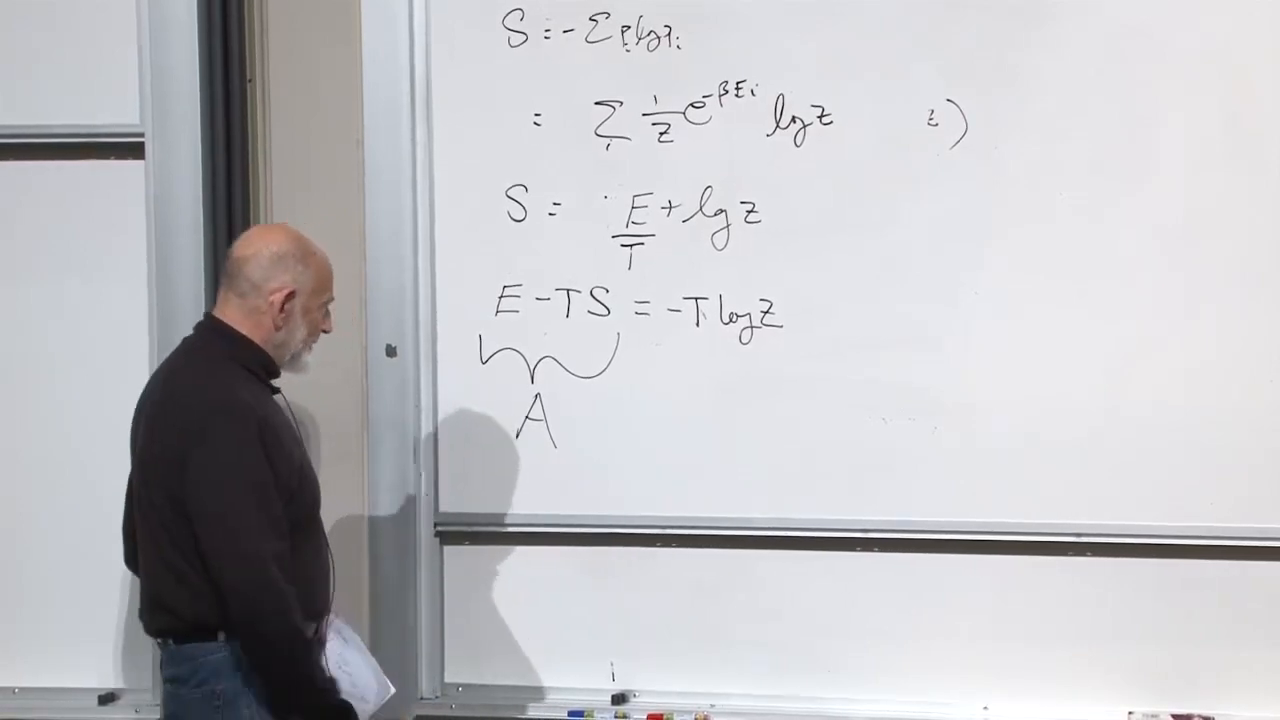
\includegraphics[width=0.90\textwidth]{lecture_05_figure_03.png}
\caption{正準エントロピー関係を\(A=E-TS=-T\log Z\)に整理したもの。}
\lectureframe{00:16:50}
\end{figure}

\section{制御パラメータとその応答}

制御パラメータとは、実験者が外部から変化させることができるマクロな量である。ピストンを動かすと、個々の分子を操作することなく体積が変化する。印加された電場や磁場も他の例である。より一般的なアンサンブルでは、粒子数も変化させることができる。

熱力学変数は自然に共役対をなす。体積は現在の問題における制御パラメータであり、圧力はその応答である。我々は\(V\)を変化させる。圧力は、系がその変化にエネルギー的にどのように抵抗するかを教えてくれる。後にエネルギーの微分がこの対を正確なものにする。

\begin{classroomqa}
\audiencequestion{圧力そのものを制御パラメータと見なせるだろうか。}
\lecturerresponse{外部圧力を固定する実験を設計することはできるが、ここで用いた構成ではピストンの位置が体積を固定し、内部圧力が応答である。圧力と体積は共役な変数であり、どちらが制御されるかはアンサンブルと装置に依存する。
\lecturetimestamp{00:19:22--00:20:01}}
\end{classroomqa}

\begin{classroomqa}
\audiencequestion{すべての分子は同一と仮定されるのか、それとも議論は気体に限られるのか。}
\lecturerresponse{熱力学の議論にはそのような制限は必要ない。シリンダーには複数の種、液体、あるいは圧縮される固体さえ入っていてよい。理想気体の分配関数は、一般的な圧力の式が確立された後に初めて特別な適用例となる。
\lecturetimestamp{00:20:02--00:20:39}}
\end{classroomqa}

\begin{classroomqa}
\audiencequestion{物質の量を別の外部操作として変化させられるだろうか。}
\lecturerresponse{はい。粒子数はもう一つの可能な制御パラメータである。それを動的に扱うと、それ自身の共役変数である化学ポテンシャルが導かれる。今夜の計算では、\(N\)は固定されたままである。
\lecturetimestamp{00:20:39--00:20:57}}
\end{classroomqa}

\begin{classroomqa}
\audiencequestion{液体の水と水蒸気が平衡状態で同時に存在できるだろうか。}
\lecturerresponse{共存温度と圧力においては存在できる。重力によって液体が蒸気の下に位置することがあるが、それでも二つの相は一つの温度を共有し、熱平衡を保つことができる。同じ一般的な統計力学の枠組みが適用される。
\lecturetimestamp{00:20:59--00:21:36}}
\end{classroomqa}

次の議論のために、エネルギーとエントロピーを二つの独立に調整可能な変数の従属関数と見なす：
\begin{equation}
 E=E(T,V),
 \qquad
 S=S(T,V).
 \label{eq:sm5-dependent-functions}
\end{equation}
温度と体積は熱力学状態空間上の座標を与える。エネルギーとエントロピーはその空間のすべての平衡点に数値を割り当てる。

\section{定エントロピー微分}

最終的に必要な微分は珍しいものである：
\[
 \left(\frac{\partial E}{\partial V}\right)_S.
\]
\(T\)と\(V\)は独立な座標であるが、この微分は従属関数\(S(T,V)\)を一定に保つよう制約しながら\(V\)を変化させることを求める。それは\((T,V)\)平面内の曲線に沿った微分であり、座標軸に沿ったものではない。

\begin{classroomqa}
\audiencequestion{後に微分\(dT/dV\)が用いられるのであれば、\(T\)と\(V\)はどのように独立でありうるのか。}
\lecturerresponse{それらは完全な状態空間上では独立である。制約\(S(T,V)=\mathrm{constant}\)を課すと、許される状態は一次元の等高線上に載る。その等高線に沿って、\(T\)は\(V\)の関数となり、その傾き\(dT/dV\)は well-defined である。
\lecturetimestamp{01:01:18--01:02:09}}
\end{classroomqa}

\begin{lemma}
\(E(T,V)\)と\(S(T,V)\)が微分可能であれば、\((\partial S/\partial T)_V\neq0\)であるところではどこでも
\begin{equation}
 \left(\frac{\partial E}{\partial V}\right)_S
 =
 \left(\frac{\partial E}{\partial V}\right)_T
 -
 \left(\frac{\partial E}{\partial S}\right)_V
 \left(\frac{\partial S}{\partial V}\right)_T.
 \label{eq:sm5-calculus-lemma}
\end{equation}
\end{lemma}

\begin{proof}
任意の無限小変位に対して、
\begin{equation}
 dE=
 \left(\frac{\partial E}{\partial V}\right)_T dV
 +
 \left(\frac{\partial E}{\partial T}\right)_V dT.
 \label{eq:sm5-total-differential-e}
\end{equation}
\(V\)を固定すると、連鎖律により\(S\)を中間変数として用いることができる：
\begin{equation}
 \left(\frac{\partial E}{\partial T}\right)_V
 =
 \left(\frac{\partial E}{\partial S}\right)_V
 \left(\frac{\partial S}{\partial T}\right)_V.
 \label{eq:sm5-chain-rule-e-s-t}
\end{equation}

ここで変位を\(S\)が一定である等高線に制限する。その等高線に沿って、
\begin{equation}
 0=dS=
 \left(\frac{\partial S}{\partial V}\right)_T dV
 +
 \left(\frac{\partial S}{\partial T}\right)_V dT.
 \label{eq:sm5-constant-entropy-differential}
\end{equation}
等高線の傾きについて解くと
\begin{equation}
 \left(\frac{dT}{dV}\right)_S
 =
 -
 \frac{\left(\frac{\partial S}{\partial V}\right)_T}
 {\left(\frac{\partial S}{\partial T}\right)_V}.
 \label{eq:sm5-entropy-contour-slope}
\end{equation}
\eqref{eq:sm5-total-differential-e}を\(dV\)で割り、
\eqref{eq:sm5-chain-rule-e-s-t}を用い、
\eqref{eq:sm5-entropy-contour-slope}を代入する：
\begin{align}
 \left(\frac{\partial E}{\partial V}\right)_S
 &=
 \left(\frac{\partial E}{\partial V}\right)_T
 +
 \left(\frac{\partial E}{\partial S}\right)_V
 \left(\frac{\partial S}{\partial T}\right)_V
 \left(\frac{dT}{dV}\right)_S \notag\\
 &=
 \left(\frac{\partial E}{\partial V}\right)_T
 -
 \left(\frac{\partial E}{\partial S}\right)_V
 \left(\frac{\partial S}{\partial V}\right)_T.
\end{align}
因子\((\partial S/\partial T)_V\)は相殺され、結果が証明される。
\end{proof}

\begin{figure}[t]
\centering
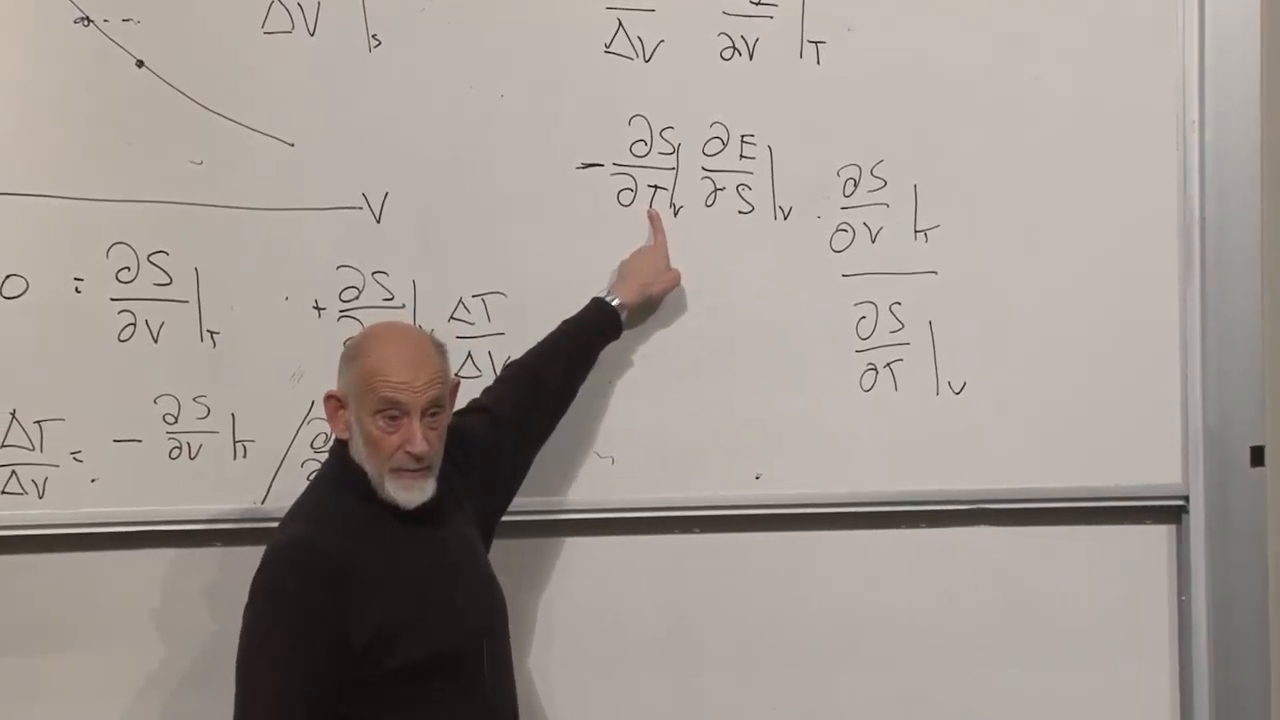
\includegraphics[width=0.90\textwidth]{lecture_05_figure_04.png}
\caption{微分補題を完成させる相殺における定エントロピー等高線の計算。}
\lectureframe{00:36:10}
\end{figure}

幾何学的な描像は装飾ではない。それは、一見奇妙な固定\(S\)微分が、独立な座標\(T\)と\(V\)における通常の偏微分で評価できる理由を説明する。構成の途中で\(\delta E/\delta V\)と書くことは、記号が指定された経路に沿った小さな変化の比を表すことを思い出させるのに有用である。

\begin{classroomqa}
\audiencequestion{\(dE\)の展開は単に偏微分の通常の定義ではないのか。}
\lecturerresponse{はい。全微分には特別なことは何も起こらない。唯一の追加要素は、後に等高線\(dS=0\)に制限することであり、それが\(dT\)と\(dV\)の関係を決定する。
\lecturetimestamp{00:29:26--00:29:32}}
\end{classroomqa}

\begin{classroomqa}
\audiencequestion{相殺には\((\partial S/\partial T)_V\)が非零であることが必要か。}
\lecturerresponse{はい。通常の安定な系では、
\[
 \left(\frac{\partial S}{\partial T}\right)_V
 =\frac{C_V}{T}>0,
\]
であるから、割り算は正当である。例外的な点には別途の注意が必要である。ハミルトニアンを固定すると、温度を上げることは正準エネルギー分布を広げ、通常はエントロピーを増加させる。温度を下げることはそれを狭める。これが単調性の議論の物理的に正しい向きである。
\lecturetimestamp{00:36:50--00:37:47}}
\end{classroomqa}

\section{ピストンの仕事と断熱条件}

ここで、この導関数に物理的な意味を与える。断面積\(\mathcal A\)のピストンを考える。これが外側へ\(dx\)だけ動くと、
\begin{equation}
 dV=\mathcal A\,dx.
 \label{eq:sm5-piston-volume}
\end{equation}
気体はピストンに力\(P\mathcal A\)を及ぼすので、気体がする仕事は
\begin{equation}
 \delta W_{\mathrm{by}}=P\mathcal A\,dx=P\,dV.
 \label{eq:sm5-piston-work}
\end{equation}
気体に熱が入らないなら、エネルギー保存により
\begin{equation}
 dE=-P\,dV.
 \label{eq:sm5-adiabatic-work}
\end{equation}
符号は物理的である。膨張の間、気体はピストンを押し上げるか加速し、自身のエネルギーは減少する。

\begin{figure}[t]
\centering
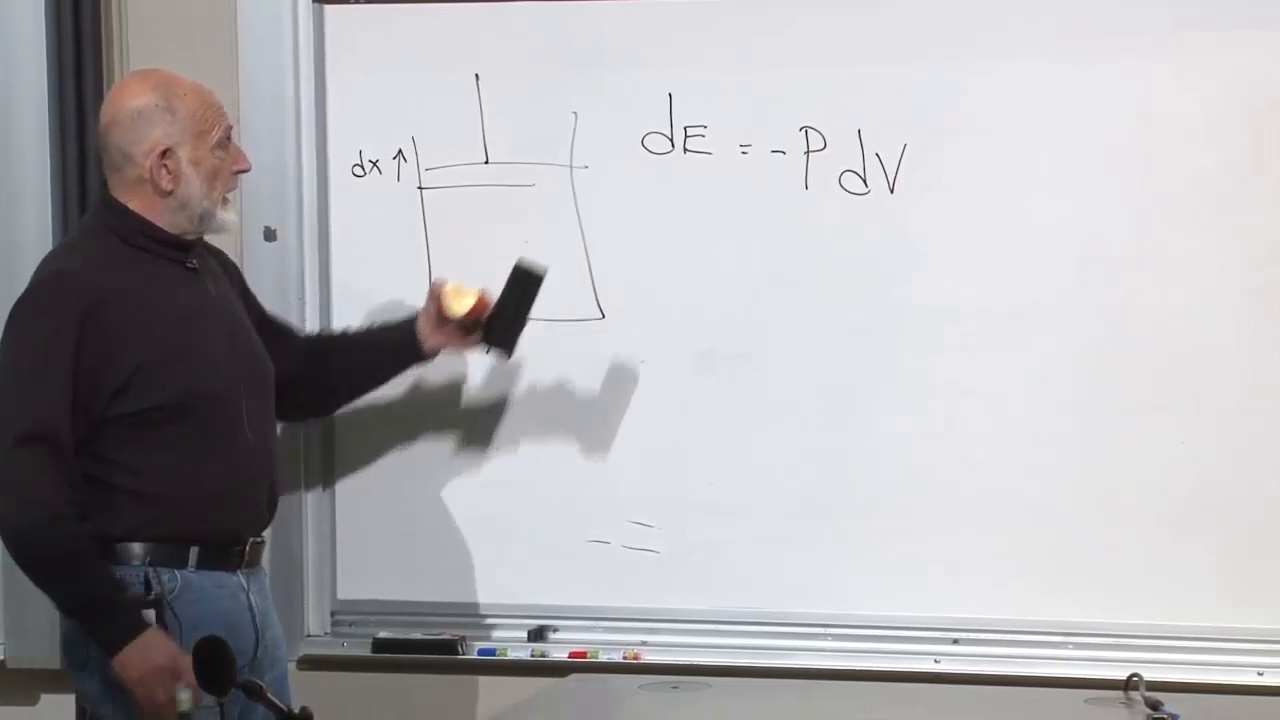
\includegraphics[width=0.90\textwidth]{lecture_05_figure_05.png}
\caption{ピストンの幾何と、完成した仕事の関係
\(dE=-P\,dV\)。}
\lectureframe{00:43:10}
\end{figure}

二つの条件が本質的である。ピストンは、系が平衡にいくらでも近いままでいられるほどゆっくり動かなければならず、また壁は断熱されていて、エネルギーが熱として供給されないようにしなければならない。急速な引き出しは、運動の間にどの分子も後退するピストンに到達しないほど速くなりうる。急速な圧縮は衝撃波を生じる。どちらの過程も、平衡状態の列では表されない。

\emph{断熱}という語は、熱移動がないことに対して使われることもあり、ゆっくりした変化に対して使われることもある。ここで要求される可逆過程では、両方の考えが入る。すなわち、変化は準静的かつ熱的に断熱されている。そのような条件下では、それは等エントロピーでもある。

\begin{classroomqa}
\audiencequestion{なぜ断熱変化はエントロピーを一定に保つのか。}
\lecturerresponse{系を量子力学的に見る。その多体エネルギー準位は体積に依存する。\(V\)がゆっくり変化するとき、断熱定理は各占有準位を、準位ラベル間の遷移なしに、連続的にその後継へ移す。エネルギー\(E_i(V)\)は動くが、占有確率\(p_i\)は固定されたままである。
\(S=-\sum_i p_i\log p_i\)はそれらの確率に依存するので、エントロピーは一定のままである。熱交換や不可逆な運動はこの結論を無効にするであろう。
\lecturetimestamp{00:43:37--00:49:15}}
\end{classroomqa}

\begin{figure}[t]
\centering
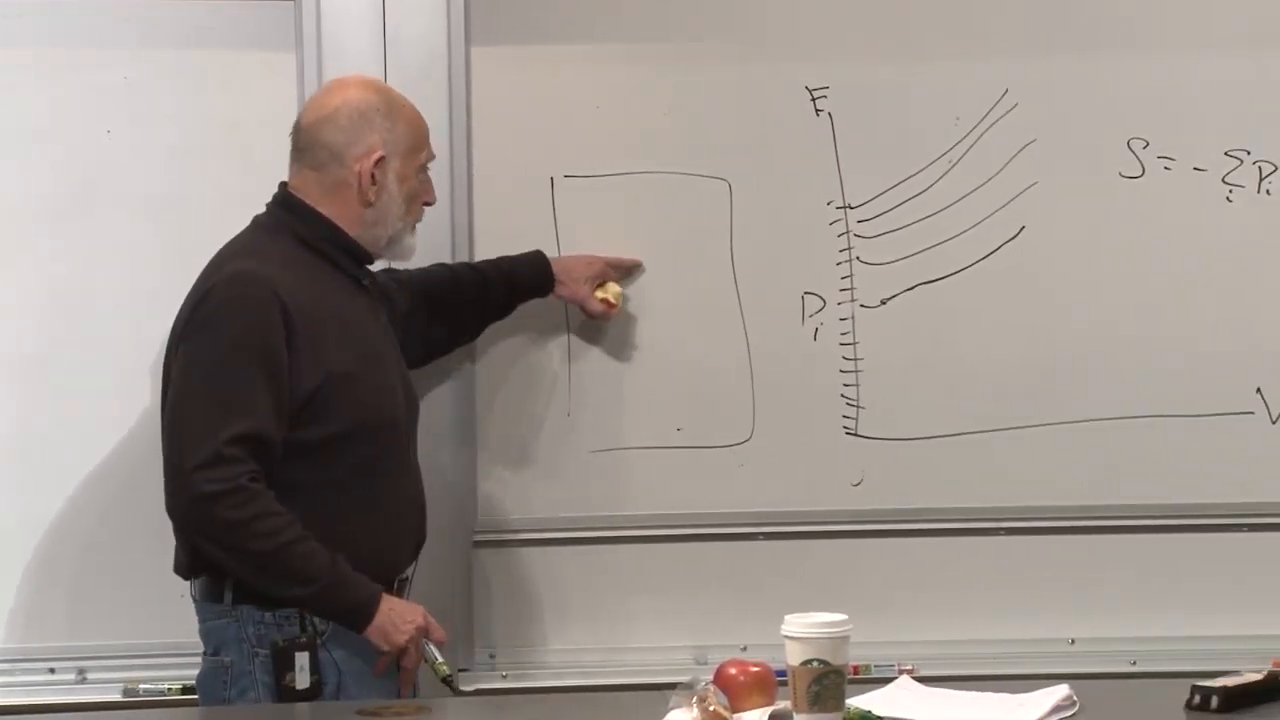
\includegraphics[width=0.90\textwidth]{lecture_05_figure_06.png}
\caption{多体エネルギー準位が体積とともに動く一方で、それらの占有確率は準位ラベルを保つ。}
\lectureframe{00:48:50}
\end{figure}

この一定エントロピーの経路に沿って評価された式\eqref{eq:sm5-adiabatic-work}は、圧力を
\begin{equation}
 P=-\left(\frac{\partial E}{\partial V}\right)_S.
 \label{eq:sm5-pressure-fixed-entropy}
\end{equation}
と同定する。これが圧力と体積の共役関係である。

\begin{classroomqa}
\audiencequestion{代わりにピストンを急速に動かすとどうなるか。}
\lecturerresponse{系は平衡を離れ、その詳細な力学が重要になる。突然の圧縮は衝撃を生じる。理想的な自由膨張では、どの分子もピストンに衝突する前にピストンが後退しうるので、仕事はなされず、体積が変化してもエネルギーは固定されたままである。気体は後に、増大したエントロピーとともに平衡へ緩和する。そのような過程は、
\eqref{eq:sm5-pressure-fixed-entropy}
における単一の平衡導関数では記述できない。
\lecturetimestamp{00:58:30--01:01:15}}
\end{classroomqa}

\begin{classroomqa}
\audiencequestion{変化がゆっくりであるかどうかを決める定量的条件は何か。}
\lecturerresponse{外部変化の時間は、関連する内部緩和時間に比べて長くなければならない。気体については、巨視的変化の間に多数の分子衝突と多数の壁への衝突が起こるべきである。正確な時間尺度は物質と幾何に依存するが、準静的極限そのものは一般的である。
\lecturetimestamp{01:02:09--01:03:20}}
\end{classroomqa}

\section{断熱エネルギーから分配関数へ}

物理的な式\eqref{eq:sm5-pressure-fixed-entropy}は、まだ計算しやすいものではない。正準統計力学は、\(T\)がボルツマン重みに直接現れるため、温度の関数を自然に与える。微積分の補題は、扱いにくい固定エントロピー導関数をその計算の言語へ変換する。
\begin{align}
 P
 &=
 -\left(\frac{\partial E}{\partial V}\right)_T
 +
 \left(\frac{\partial E}{\partial S}\right)_V
 \left(\frac{\partial S}{\partial V}\right)_T.
 \label{eq:sm5-pressure-lemma-substitution}
\end{align}
固定体積では、第一法則は\(dE=T\,dS\)を与えるので、
\begin{equation}
 \left(\frac{\partial E}{\partial S}\right)_V=T.
 \label{eq:sm5-e-s-temperature}
\end{equation}
したがって
\begin{equation}
 P=
 -\left(\frac{\partial E}{\partial V}\right)_T
 +
 T\left(\frac{\partial S}{\partial V}\right)_T.
 \label{eq:sm5-pressure-fixed-temperature-pieces}
\end{equation}

\begin{classroomqa}
\audiencequestion{圧力の式のマイナス符号はどこから来るのか。}
\lecturerresponse{それは気体がする仕事に由来する。
\(dE=-P\,dV\)（断熱膨張の間）。微積分の補題自体はその二つの項の間にマイナス符号をもつ。
\(P=-(\partial E/\partial V)_S\)
における全体のマイナスはそれら両方を反転させ、
\eqref{eq:sm5-pressure-fixed-temperature-pieces}
を生じる。
\lecturetimestamp{00:52:40--00:53:14}}
\end{classroomqa}

\(T\)は両方の導関数で固定されているので、
\begin{align}
 P
 &=
 -\left(\frac{\partial}{\partial V}(E-TS)\right)_T \notag\\
 &=
 -\left(\frac{\partial A}{\partial V}\right)_T.
 \label{eq:sm5-pressure-free-energy}
\end{align}
最後に\(A=-T\log Z\)を代入する。
\begin{equation}
 \boxed{
 P=
 T\left(\frac{\partial\log Z}{\partial V}\right)_T
 }.
 \label{eq:sm5-pressure-log-z}
\end{equation}

\begin{figure}[t]
\centering
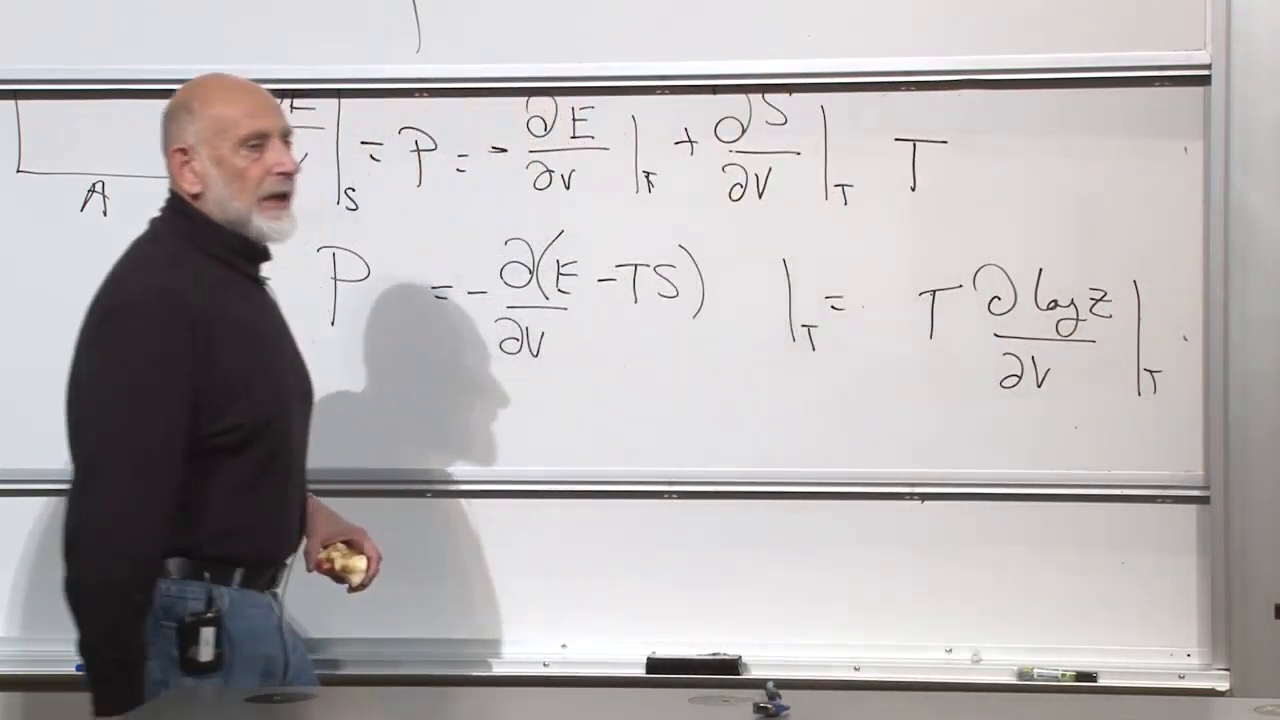
\includegraphics[width=0.90\textwidth]{lecture_05_figure_07.png}
\caption{引数の固定温度圧縮：
\(P=-(\partial A/\partial V)_T
=T(\partial\log Z/\partial V)_T\)。}
\lectureframe{00:55:55}
\end{figure}

\eqref{eq:sm5-pressure-log-z}のどこにも理想気体は仮定されていない。相互作用する流体、プラズマ、または固体について分配関数を計算できるなら、同じ導関数がその圧力を与える。より一般に、すべての外部制御パラメータは、適切な熱力学ポテンシャルを微分して得られる共役応答をもつ。分配関数はそのような応答を多数まとめ上げる。\(\log Z\)を\(\beta\)で微分するとエネルギーを与え、体積で微分すると圧力を与える。

\section{理想気体の状態方程式}

ここで初めて\(N\)個の非相互作用粒子の場合に限定する。古典的な相空間の規格化を保持したままだと、
\begin{equation}
 Z_N=
 \frac{1}{N!h^{3N}}
 \int d^{3N}q\,d^{3N}p\,
 \exp\!\left[
 -\beta\sum_{a=1}^{N}\frac{\mathbf p_a^2}{2m}
 \right].
 \label{eq:sm5-ideal-gas-partition-integral}
\end{equation}
位置座標が\(3N\)個、運動量座標が\(3N\)個ある。ハミルトニアンは位置に依存しないので、各粒子が容器の体積の因子を1つずつ寄与する：
\begin{equation}
 Z_N=
 \frac{V^N}{N!h^{3N}}I_p(\beta),
 \label{eq:sm5-ideal-gas-factorization}
\end{equation}
ここで運動量積分全体\(I_p(\beta)\)は\(V\)に依存しない。

\begin{classroomqa}
\audiencequestion{なぜ位置積分が\(3N\)個、運動量積分が\(3N\)個あるのか。}
\lecturerresponse{\(N\)個の粒子のそれぞれが3つの空間座標と3つの共役な運動量成分をもつ。その数は相空間の各半分で\(3N\)であり、\(N\)個の粒子にさらに\(3N\)個の粒子が加わるのではない。
\lecturetimestamp{01:04:19--01:04:28}}
\end{classroomqa}

対数をとると体積依存性が分離される：
\begin{equation}
 \log Z_N
 =
 N\log V-\log N!-3N\log h+\log I_p(\beta).
 \label{eq:sm5-log-ideal-gas-partition}
\end{equation}
因子\(1/N!\)、\(h^{-3N}\)、\(I_p(\beta)\)はすべて体積に依存しない。これらは絶対エントロピーやその他の問題には重要だが、この特定の導関数には重要でない。したがって
\begin{equation}
 \left(\frac{\partial\log Z_N}{\partial V}\right)_T
 =\frac{N}{V}.
 \label{eq:sm5-log-z-volume-derivative}
\end{equation}
式\eqref{eq:sm5-pressure-log-z}から直ちに
\begin{equation}
 P=\frac{NT}{V},
 \qquad
 \boxed{PV=NT}.
 \label{eq:sm5-ideal-gas-law}
\end{equation}が得られる。

\begin{classroomqa}
\audiencequestion{\(N\)はボルツマン分布を導出するのに用いたレプリカを依然として数えているのか。}
\lecturerresponse{いいえ。レプリカの構成は以前の導出における数え上げの道具であり、もはや存在しない。ここで\(N\)はこの1つの気体試料中の物理的粒子の数である。
\lecturetimestamp{01:07:38--01:08:05}}
\end{classroomqa}

数密度を
\begin{equation}
 \rho=\frac{N}{V}
 \label{eq:sm5-number-density}
\end{equation}
と定義すると、等価な形
\begin{equation}
 P=\rho T.
 \label{eq:sm5-density-equation-of-state}
\end{equation}が得られる。

\begin{classroomqa}
\audiencequestion{密度の形は\(N\)で割るのか、それとも\(V\)で割るのか。}
\lecturerresponse{\(PV=NT\)を\(V\)で割る：
\(P=(N/V)T=\rho T\)。ここで\(\rho\)は数密度であり、質量密度ではない。
\lecturetimestamp{01:08:45--01:09:16}}
\end{classroomqa}

\begin{figure}[t]
\centering
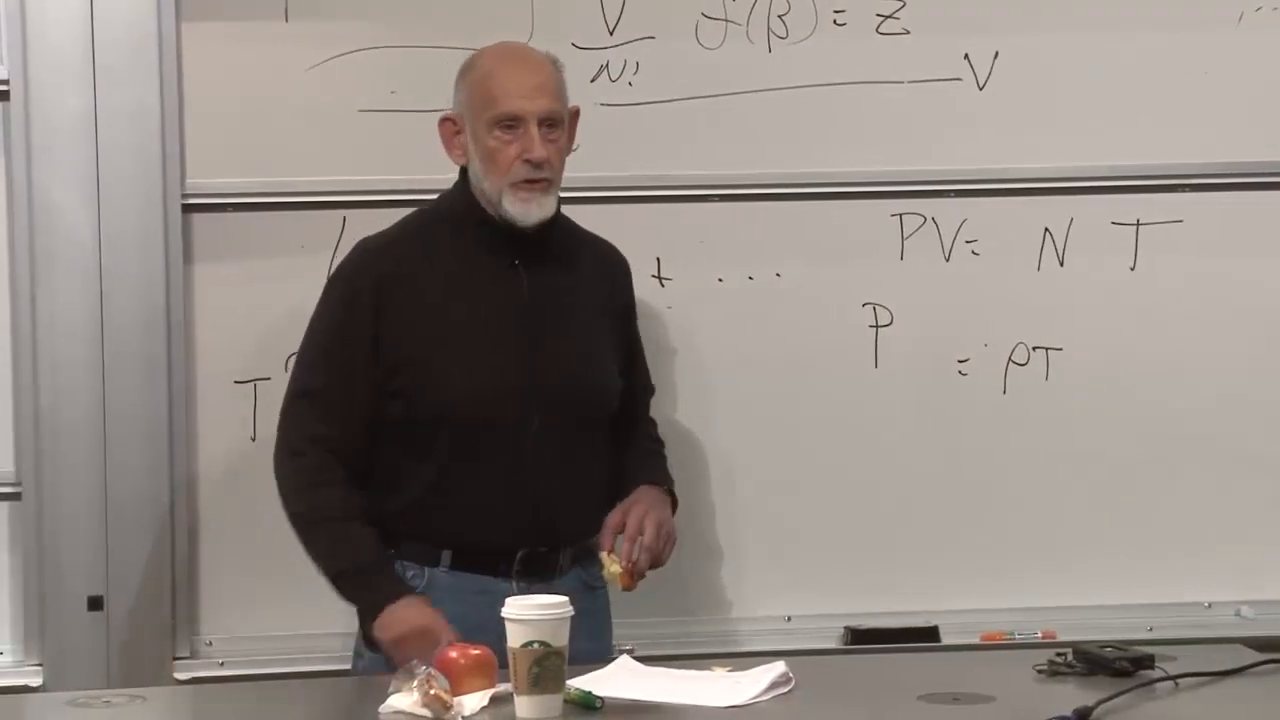
\includegraphics[width=0.90\textwidth]{lecture_05_figure_08.png}
\caption{\(\log Z\)の体積導関数と、それから得られる理想気体の状態方程式\(PV=NT\)、すなわち\(P=\rho T\)。}
\lectureframe{01:09:25}
\end{figure}

実験室温度\(T_K\)を復元すると、
\begin{equation}
 PV=Nk_BT_K.
 \label{eq:sm5-ideal-gas-law-laboratory}
\end{equation}
このよく知られた結果は運動論的な直観と一致するが、その導出は今や自由気体をはるかに超えて生き残る枠組みに基づいている。

\section{第二の配当：平衡揺らぎ}

圧力の計算は完了したが、約束した問いが1つ残っている：分配関数から他に何を引き出せるか。熱浴と熱接触している系を考える。そのエネルギーは固定されていない。エネルギーが出入りするので、繰り返しの測定はカノニカル平均の周りで揺らぐ。

\begin{classroomqa}
\audiencequestion{約束された揺らぎを今計算できるか。}
\lecturerresponse{はい。余分な時間によって同じ原理の第二の実演が可能になる：\(Z\)の導関数が測定可能な熱力学的情報を符号化している。
\lecturetimestamp{01:10:37--01:10:50}}
\end{classroomqa}

\subsection{分散と標準偏差}

\(\langle x\rangle=0\)をもつ確率変数\(x\)に対して、分布の幅の尺度は\(\langle x^2\rangle\)である。一般の分布に対しては、変数をその平均だけずらす：
\begin{equation}
 \delta x=x-\langle x\rangle.
 \label{eq:sm5-centered-variable}
\end{equation}
その平均は消え、
\begin{equation}
 \langle\delta x\rangle
 =
 \langle x\rangle-\langle x\rangle=0,
 \label{eq:sm5-centered-mean}
\end{equation}
その平均二乗は
\begin{align}
 (\Delta x)^2
 &\equiv
 \left\langle\left(x-\langle x\rangle\right)^2\right\rangle \notag\\
 &=
 \langle x^2\rangle
 -2\langle x\rangle^2
 +\langle x\rangle^2 \notag\\
 &=
 \langle x^2\rangle-\langle x\rangle^2.
 \label{eq:sm5-variance}
\end{align}
これが分散である。その正の平方根\(\Delta x\)が標準偏差である。

\begin{classroomqa}
\audiencequestion{なぜ
\(x-\langle x\rangle\)の平均がちょうどゼロなのか。}
\lecturerresponse{平均は線形であり、\(\langle x\rangle\)はすでに数である。したがって
\(\langle x-\langle x\rangle\rangle
=\langle x\rangle-\langle x\rangle=0\)。
\lecturetimestamp{01:14:02--01:14:22}}
\end{classroomqa}

\begin{classroomqa}
\audiencequestion{二乗揺らぎ、分散、二乗平均平方根幅、標準偏差の区別は何か。}
\lecturerresponse{分散は
\((\Delta x)^2=\langle x^2\rangle-\langle x\rangle^2\)。
標準偏差はその平方根\(\Delta x\)である。平均がゼロの変数では、標準偏差はその二乗平均平方根値でもある。
\lecturetimestamp{01:16:39--01:18:38}}
\end{classroomqa}

\begin{figure}[t]
\centering
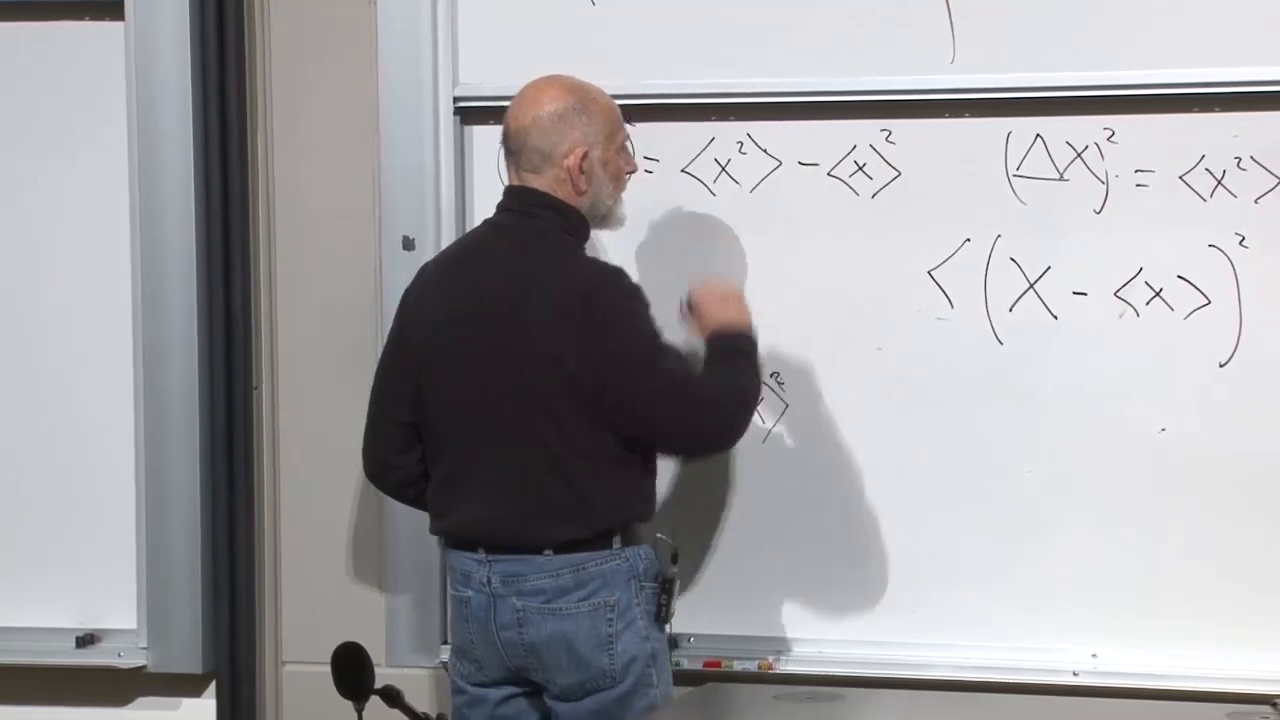
\includegraphics[width=0.90\textwidth]{lecture_05_figure_09.png}
\caption{ずらした変数と、\((\Delta x)^2=\langle x^2\rangle-\langle x\rangle^2\)を生み出す展開。}
\lectureframe{01:17:20}
\end{figure}

\subsection{分配関数からのエネルギーモーメント}

カノニカル集団では、
\begin{align}
 \langle E\rangle
 &=
 \frac{1}{Z}\sum_i E_i e^{-\beta E_i} \notag\\
 &=
 -\frac{1}{Z}\frac{\partial Z}{\partial\beta}
 =
 -\frac{\partial\log Z}{\partial\beta}.
 \label{eq:sm5-mean-energy-from-z}
\end{align}
\(E_i\)の因子1つ分の掛け算は、1つの負の\(\beta\)導関数によって生み出される。2階導関数は\(E_i^2\)を生成する：
\begin{equation}
 \langle E^2\rangle
 =
 \frac{1}{Z}\sum_i E_i^2e^{-\beta E_i}
 =
 \frac{1}{Z}\frac{\partial^2 Z}{\partial\beta^2}.
 \label{eq:sm5-second-energy-moment}
\end{equation}
したがってエネルギーの分散は
\begin{align}
 (\Delta E)^2
 &=
 \langle E^2\rangle-\langle E\rangle^2 \notag\\
 &=
 \frac{1}{Z}\frac{\partial^2Z}{\partial\beta^2}
 -
 \frac{1}{Z^2}
 \left(\frac{\partial Z}{\partial\beta}\right)^2 \notag\\
 &=
 \frac{\partial^2\log Z}{\partial\beta^2}
 =
 -\frac{\partial\langle E\rangle}{\partial\beta}.
 \label{eq:sm5-energy-variance-beta}
\end{align}
ここでもまた、複雑に見える観測量が\(\log Z\)の導関数になる。

\begin{figure}[t]
\centering
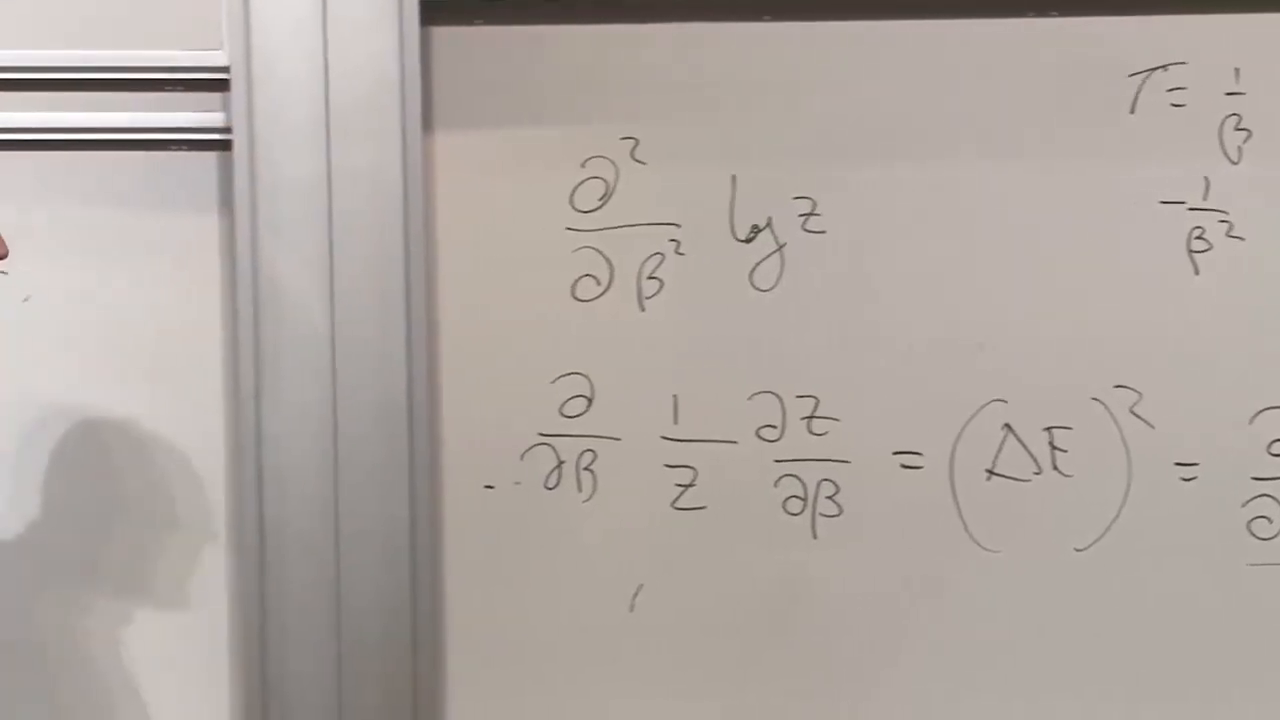
\includegraphics[width=0.90\textwidth]{lecture_05_figure_10.png}
\caption{\(\log Z\)の2階\(\beta\)導関数をエネルギーの分散と同定したもの。}
\lectureframe{01:29:00}
\end{figure}

\subsection{熱容量と揺らぎの大きさ}

講義単位では\(T=1/\beta\)なので、
\begin{equation}
 -\frac{\partial}{\partial\beta}
 =
 T^2\frac{\partial}{\partial T}.
 \label{eq:sm5-beta-temperature-derivative}
\end{equation}
体積を固定して、試料全体の熱容量を
\begin{equation}
 C_V\equiv
 \left(\frac{\partial\langle E\rangle}{\partial T}\right)_V.
 \label{eq:sm5-heat-capacity}
\end{equation}
と定義する。式\eqref{eq:sm5-energy-variance-beta}は
\begin{equation}
 \boxed{(\Delta E)^2=T^2C_V}
 \qquad (k_B=1).
 \label{eq:sm5-energy-fluctuation-lecture-units}
\end{equation}
となる。実験室温度\(T_K\)では、ここで
\(\beta=(k_BT_K)^{-1}\)、
\begin{equation}
 \boxed{(\Delta E)^2=k_BT_K^2C_V}.
 \label{eq:sm5-energy-fluctuation-laboratory}
\end{equation}

\begin{figure}[t]
\centering
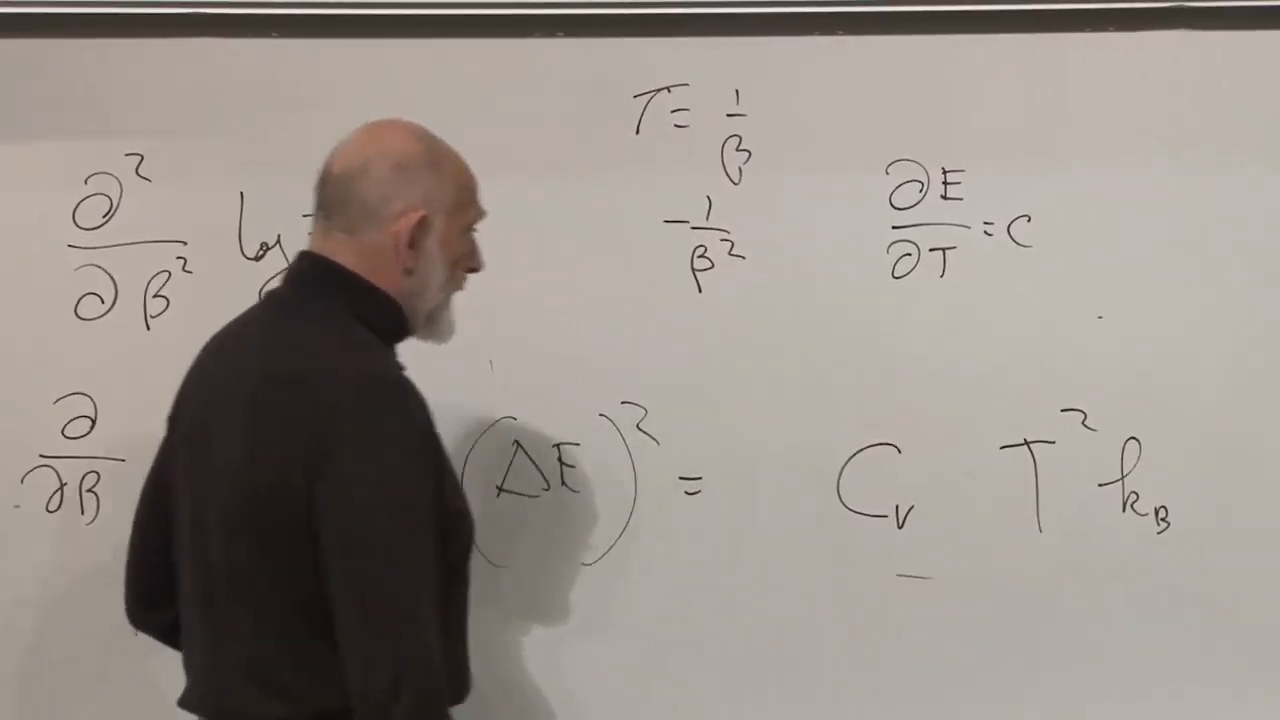
\includegraphics[width=0.90\textwidth]{lecture_05_figure_11.png}
\caption{\(\beta\) 微分から定積熱容量への変換。ただし、復元された \(k_B\) の因子を含む。}
\lectureframe{01:31:10}
\end{figure}

\begin{classroomqa}
\audiencequestion{微分は定圧ではなく定積を指定しなければならないのか。}
\lecturerresponse{はい。この正準分布による導出では、ハミルトニアンの外部制御パラメータを \(V\) を含めて固定したままにする。得られる量は \(C_V\) である。定圧アンサンブルでは体積と仕事が揺らぐことが許され、対応する熱力学ポテンシャルが必要となる。\eqref{eq:sm5-energy-fluctuation-laboratory} において \(C_V\) を単に \(C_P\) に置き換えることはできない。
\lecturetimestamp{01:29:01--01:29:28; 01:32:50--01:33:21}}
\end{classroomqa}

\begin{classroomqa}
\audiencequestion{\(C_V\) は物質定数か。}
\lecturerresponse{一般にはそうではない。温度、体積、相、組成に依存しうる。さらに、ここでの \(C_V\) は試料全体の熱容量であり、示量的である。比熱は質量、粒子数、または物質量で割って初めて得られる。
\lecturetimestamp{01:31:47--01:32:21; 01:33:23--01:34:55}}
\end{classroomqa}

通常の示量的な物質では、\(C_V\) は \(N\) に比例するので、\((\Delta E)^2\) は \(N\) に比例し、\(\Delta E\) は \(\sqrt{N}\) に比例する。平均エネルギー自体も \(N\) に比例する。したがって
\begin{equation}
 \frac{\Delta E}{\langle E\rangle}\sim\frac{1}{\sqrt{N}}.
 \label{eq:sm5-relative-fluctuation-scaling}
\end{equation}
巨視的な相対揺らぎはきわめて小さく、一方で微視的な試料ではそれが直接現れる。\eqref{eq:sm5-energy-fluctuation-laboratory} に \(k_B\) が現れることは、熱力学の観測量と分子の離散性とのこの結びつきを示しており、同等に、巨視的な単位をアボガドロ規模の計数に結びつけている。

圧力と揺らぎは今や同じ対象から現れた：
\[
 P=T\left(\frac{\partial\log Z}{\partial V}\right)_T,
 \qquad
 (\Delta E)^2=\frac{\partial^2\log Z}{\partial\beta^2}.
\]
これが中心的な教訓である。正しい拘束条件を特定しさえすれば、分配関数は単に確率を規格化するだけではない。その導関数が系の測定可能な熱力学を組織する。